%**************************************************************************************
% License:
% CC BY-NC-SA 4.0 (http://creativecommons.org/licenses/by-nc-sa/4.0/)
%**************************************************************************************

\documentclass[notes]{beamer}

\mode<presentation> {

\usetheme{Madrid}

% Burnt orange
\definecolor{burntorange}{rgb}{0.8, 0.33, 0.0}
\colorlet{beamer@blendedblue}{burntorange}
% Pale yellow
\definecolor{paleyellow}{rgb}{1.0, 1.0, 0.953}
\setbeamercolor{background canvas}{bg=paleyellow}
% Secondary and tertiary palett
\setbeamercolor*{palette secondary}{use=structure,fg=white,bg=burntorange!80!black}
\setbeamercolor*{palette tertiary}{use=structure,fg=white,bg=burntorange!60!black}

% To remove the footer line in all slides uncomment this line
%\setbeamertemplate{footline}
% To replace the footer line in all slides with a simple slide count uncomment this line
%\setbeamertemplate{footline}[page number]

% To remove the navigation symbols from the bottom of all slides uncomment this line
%\setbeamertemplate{navigation symbols}{}
}

\usepackage{amsmath}
\usepackage{bm}
\usepackage{breqn}
\usepackage{cancel}
\usepackage{graphicx} % for figures
\usepackage{subcaption} % for subplots 
\usepackage[labelsep=space,tableposition=top]{caption}
\renewcommand{\figurename}{Fig.} 
\usepackage{cleveref}
\usepackage{caption,subcaption}% http://ctan.org/pkg/{caption,subcaption}
\usepackage{booktabs} % Allows the use of \toprule, \midrule and \bottomrule in tables
\usepackage{multirow}
\usepackage{tabularx}

% To print 2 slides on a page
%\usepackage{handoutWithNotes}
%\pgfpagesuselayout{2 on 1}[border shrink=2mm]
%----------------------------------------------------------------------------------------
%	TITLE PAGE
%----------------------------------------------------------------------------------------
% The short title appears at the bottom of every slide, the full title is only on the title page
\title[CE394M: Linear Elasticity]{CE394M: Linear Elasticity} 
\author{Krishna Kumar} % name
\institute[UT Austin] % institution 
{
University of Texas at Austin \\
\medskip
\textit{
  \url{krishnak@utexas.edu}} % Your email address
}
\date{} % Date, can be changed to a custom date

\begin{document}

\begin{frame}
\titlepage % title page as the first slide
\end{frame}

\AtBeginSection[]
{
	\begin{frame}<beamer>
		\frametitle{Overview}
		\tableofcontents[currentsection]
	\end{frame}
}
%----------------------------------------------------------------------------------------
% slides
%----------------------------------------------------------------------------------------
\section{Linear Elasticity}
%----------------------------------------------------------------------------------------
\begin{frame}
\frametitle{Isotropic linear elastic stress-strain relations}
The relationship between the stress and strain tensor is a linear one. The stress component
is a linear combination of the strain tensor. The most general form for \textit{linear} stress-strain relations for a \textit{Cauchy elastic}
material is given by:
\mode<beamer>{
	\begin{equation*}
		\sigma_{ij} = \sigma^0_{ij} + D_{ijkl} \varepsilon_{kl}
	\end{equation*}
}
\mode<handout>{
	\vspace{2cm}
} 
	Where $\sigma^0_{ij}$ is the components of initial stress tensor corresponding to the initial strain free (when all strain components $\varepsilon_{kl} = 0$). $D_{ijkl}$ is the tensor of material \textit{elastic constants}.
	
	If it is assumed that the initial strain free state corresponds to an \textit{initial stress free state}, that is $\sigma^0_{ij} = 0$, the equations reduces to:
\mode<beamer>{	
	\begin{equation*}
		\sigma_{ij} = D_{ijkl} \varepsilon_{kl}
	\end{equation*}
}  
\mode<handout>{
	\vspace{1.5cm}
} 
\end{frame}

%----------------------------------------------------------------------------------------
\begin{frame}
\frametitle{Observation on linear elasticity}
	\begin{enumerate}
		\item $\sigma_{ij} = D_{ijkl} \varepsilon_{kl}$ is a general expression relating stress to strains for a linear solid.
		\item $D_{ijkl}$ is a 4th order tensor containing 81 terms (we trick using symmetry and reduce order).
		\item $D_{ijkl}$ material response functions having dimensions $F/L^2$.
		\item Homogeneous: $D_{ijkl}$ independent of position
		\item Isotropic: $D_{ijkl}$ independent of frame of reference.
		\item Because the stress is symmetric: $\sigma_{ij} = \sigma_{ji}$, $D_{ijkl} = D_{jikl}$. Strain is symmetric $\varepsilon_{kl} = \varepsilon_{lk}$ and $D_{ijkl} = D_{ijlk}$. Hence the number of independent variables drop from 81 to 36. 
		\item Both the stress and the strain tensor have only 6 independent values, therefor write them as vectors, then the stiffness tensor can be written as a matrix (compromise I can not rotate tensor).
	\end{enumerate}
\end{frame}

%----------------------------------------------------------------------------------------
\begin{frame}
\frametitle{Stress-strain relationship}
\begin{equation*}
\begin{bmatrix}
	\sigma_{11} \\
	\sigma_{22} \\
	\sigma_{33} \\
	\sigma_{12} \\
	\sigma_{23} \\
	\sigma_{31} \\
\end{bmatrix} %
= %
\begin{bmatrix}
	D_{11} & D_{12} & D_{13} & D_{14} &   D_{15} & D_{16}\\
	D_{21} & D_{22} & D_{23} & D_{24} &   D_{25} & D_{26}\\
	D_{31} & D_{32} & D_{33} & D_{34} &   D_{35} & D_{36}\\
	D_{41} & D_{42} & D_{43} & D_{44} &   D_{45} & D_{46}\\
	D_{51} & D_{52} & D_{53} & D_{54} &   D_{55} & D_{56}\\
	D_{61} & D_{62} & D_{63} & D_{64} &   D_{65} & D_{66}\\
\end{bmatrix} %
\begin{bmatrix}
\varepsilon_{11} \\
\varepsilon_{22} \\
\varepsilon_{33} \\
\varepsilon_{12} \\
\varepsilon_{23} \\
\varepsilon_{31} \\
\end{bmatrix}
\end{equation*}
$D_{ijkl}$ is a tensor of material \textit{elastic constants}. However, the above $[\mathbf{D}]$ is not a tensor anymore. So we can not rotate the matrix to another frame of reference. This relationship is useful for isotropic materials, where $\mathbf{D}$ is independent of the frame of reference. 
\mode<beamer>{
	\begin{equation*}
		\left\{\sigma\right\} = \left[\mathbf{D}\right]\left\{\varepsilon\right\}
	\end{equation*}
}
\mode<handout>{
	\vspace{1cm}
}
The inverse of the relationship (Compliance matrix): 
\mode<beamer>{
	\begin{equation*}
	\left\{\varepsilon\right\} = \left[\mathbf{C}\right]\left\{\sigma\right\}
	%
	\qquad 
	%
	 \left[\mathbf{C}\right] = \left[\mathbf{D}\right]^{-1}
	\end{equation*}
}
\mode<handout>{
	\vspace{1cm}
}
\end{frame}

%----------------------------------------------------------------------------------------
\begin{frame}
\frametitle{Hooke's law}
\noindent
\fboxsep=0pt
\noindent
\begin{minipage}[t]{0.89\linewidth}
	Empirical observation:
	\mode<beamer>{
		\begin{equation*}
			\Delta \varepsilon_a = \Delta \sigma_{axial} \cdot \frac{1}{E} \rightarrow \Delta \varepsilon_{11} = \frac{\Delta \sigma_{11}}{E}
		\end{equation*}
	}
	\mode<handout>{
		\vspace{1.5cm}
	}
	Where $E$ is defined as the \textit{Young's modulus}.

	The lateral strains are defined as:
	\mode<beamer>{
		\begin{align*}
			\Delta \varepsilon_{22} & = - \nu \Delta \varepsilon_{11} \\
			\Delta \varepsilon_{33} & = - \nu \Delta \varepsilon_{11}
		\end{align*}
	}
	\mode<handout>{
		\vspace{2cm}
	}

	Using superposition for principal stresses:
		\begin{align*}
			\varepsilon_{11} & = (1/E)\left[\sigma_{11} - \nu \sigma_{22} -\nu \sigma_{33}\right] \\
			%
			\varepsilon_{22} & = (1/E)\left[-\nu \sigma_{11} + \sigma_{22} -\nu \sigma_{33}\right] \\
			%
			\varepsilon_{33} & = (1/E)\left[-\nu \sigma_{11} - \nu \sigma_{22} + \sigma_{33}\right]
		\end{align*}
\end{minipage}%
\hfill%
\begin{minipage}[t]{0.1\linewidth}
	\begin{figure}
		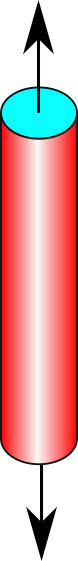
\includegraphics[width=0.8\textwidth]{figs/hookes-law.png}
	\end{figure}
\end{minipage}	
\end{frame}

%----------------------------------------------------------------------------------------
\begin{frame}
\frametitle{Hooke's law}

\begin{equation*}
	\begin{Bmatrix}
		\varepsilon_{11}\\
		\varepsilon_{22}\\
		\varepsilon_{33}\\
	\end{Bmatrix} = \frac{1}{E}
	\begin{bmatrix}
		1 & -\nu & -\nu \\
		-\nu & 1 & -\nu \\
		-\nu & -\nu & 1 \\
	\end{bmatrix}
	\begin{Bmatrix}
		\sigma_{11}\\
		\sigma_{22}\\
		\sigma_{33}\\
	\end{Bmatrix}
\end{equation*}

It is possible to invert the matrix to obtain the generalized Hooke's law: \mode<beamer>{$[\sigma] = [\mathbf{D}][\varepsilon]$.}

\begin{equation*}
	\begin{Bmatrix}
		\sigma_{11}\\
		\sigma_{22}\\
		\sigma_{33}\\
		\sigma_{12}\\
		\sigma_{13}\\
		\sigma_{23}\\
	\end{Bmatrix} = \alpha
	\begin{bmatrix}
		(1-\nu) & \nu & \nu & 0 & 0 & 0 \\
	   			& (1-\nu) & \nu & 0 & 0 & 0 \\
	   			&  & (1-\nu) & 0 & 0 & 0 \\
	   			&  & & \frac{(1-2\nu)}{2} & 0 & 0 \\
	   			&  & & & \frac{(1-2\nu)}{2}  & 0 \\
	   			&  & & & & \frac{(1-2\nu)}{2} \\
	\end{bmatrix}
	\begin{Bmatrix}
		\varepsilon_{11}\\
		\varepsilon_{22}\\
		\varepsilon_{33}\\
		2\varepsilon_{12}\\
		2\varepsilon_{13}\\
		2\varepsilon_{23}\\
	\end{Bmatrix}
\end{equation*}
Where $\alpha = E / ((1+\nu)(1-2\nu))$.
Similarly, we can obtain the inverse matrix.
\end{frame}


%----------------------------------------------------------------------------------------
\begin{frame}
\frametitle{Hooke's law}
The matrices $[\mathbf{C}]$ and $[\mathbf{D}]$ contains two indepdent variables $E$ and $\mu$, where $E > 0$ and $-1 \le \nu \le 0.5$. 
The matrix can also be defined in terms of Lame's constants.
\begin{equation*}
	\begin{cases}
		\lambda = \frac{E \nu}{(1+\nu)(1-2\nu)} \quad \text{Lame's modulus (wave propagation)}\\
		\mu = G = \frac{E}{2(1+\nu)}
		\quad \text{Shear modulus (shear behavior)}\\
		K = \frac{E}{3(1-2\nu)}
		\quad \text{Bulk modulus (volumetric behavior)}\\
	\end{cases}
\end{equation*}
\end{frame}

%----------------------------------------------------------------------------------------
\begin{frame}
\frametitle{Isotropic linear elastic}
	\begin{figure}
		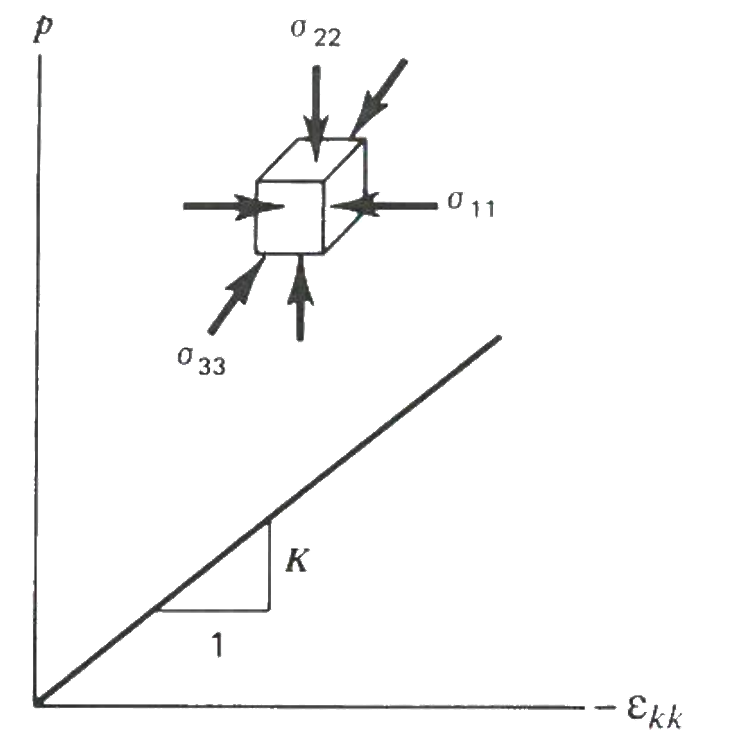
\includegraphics[width=0.95\textwidth]{figs/isotropic-linear-elastic.png}
		\caption*{Behavior of isotropic linear elastic material in simple tests: (a) hydrostatic compression test ($\sigma_{11} = \sigma_{22} = \sigma_{33} = p$) and (b) simple tension test (Chen 1994)}
	\end{figure}
\end{frame}

%----------------------------------------------------------------------------------------
\begin{frame}
\frametitle{Isotropic linear elastic}
\textbf{Hydrostatic compression test}
The non-zero components of stress: \mode<beamer>{$\sigma_{11} = \sigma_{22} = \sigma_{33} = -p = \sigma_{kk}/3$.}

The \textit{Bulk modulus, K,}  is defined as the ratio between the \textit{hydrostatic pressure p} nd the corresponding volume change $\delta \varepsilon_v = \varepsilon_{kk}$. 
\mode<beamer>{	
	\begin{equation*}
		K = - \frac{p}{\varepsilon_{kk}} = \lambda + \frac{2}{3}\mu
	\end{equation*}
}  
\mode<handout>{
	\vspace{1.5cm}
} 
\textbf{Simple tension test}
The only non-zero components of stress: \mode<beamer>{$\sigma_{11} = \sigma$}

The \textit{Young's modulus, E,}  and \textit{Poisson's ratio, $\nu$} as. 
\mode<beamer>{	
	\begin{equation*}
	E = \frac{\sigma_{11}}{\varepsilon_{11}} \quad
	\nu = \frac{-\varepsilon_{22}}{\varepsilon_{11}} = \frac{-\varepsilon_{33}}{\varepsilon_{11}}
	\end{equation*}
}  
\mode<handout>{
	\vspace{1.5cm}
}
\end{frame}

%----------------------------------------------------------------------------------------
\begin{frame}
\frametitle{Isotropic linear elastic}
\begin{figure}
	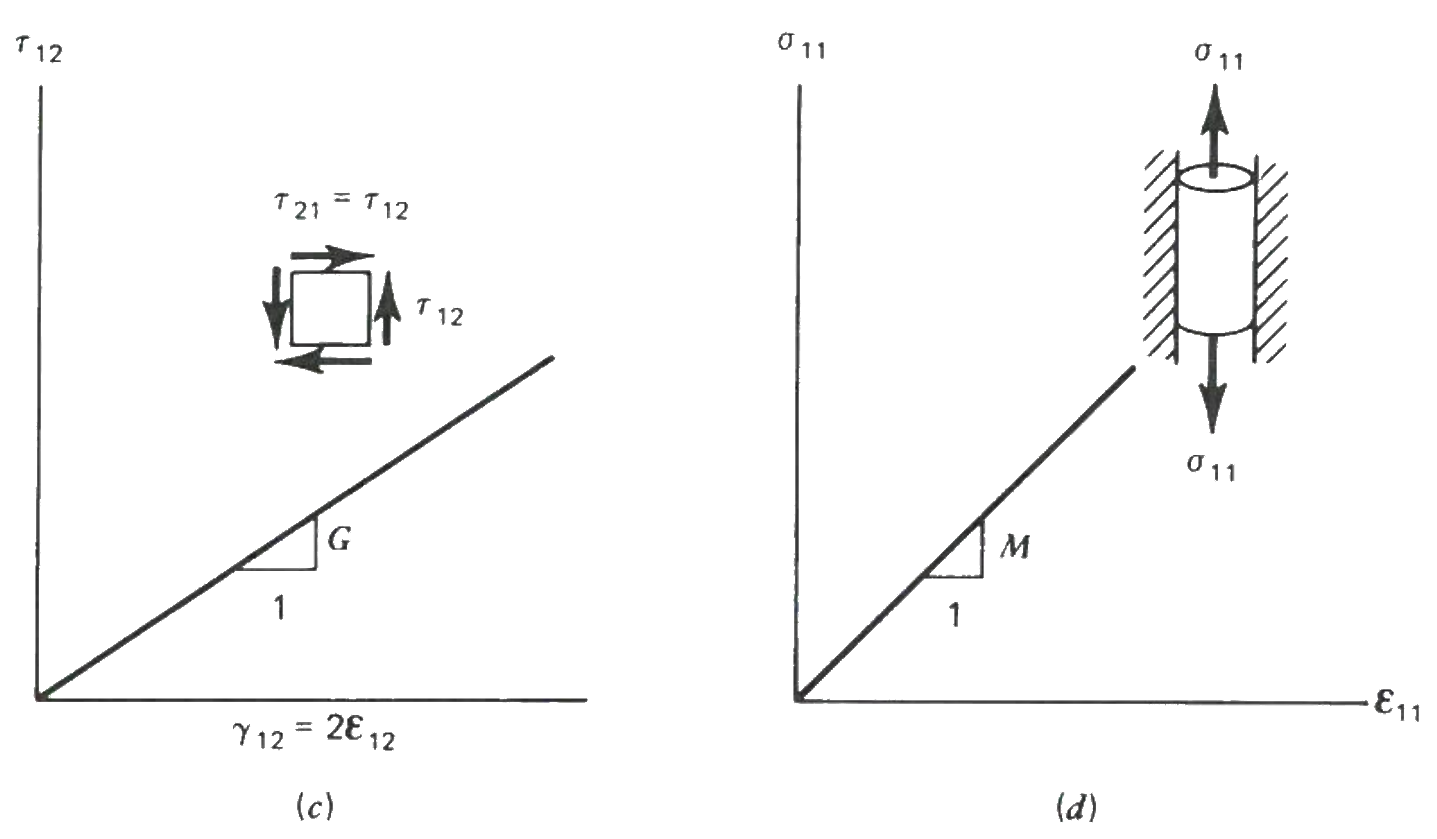
\includegraphics[width=0.95\textwidth]{figs/isotropic-linear-elastic-1.png}
	\caption*{Behavior of isotropic linear elastic material in simple tests: (c) pure shear test, and (d) uniaxial strain test (Chen 1994)}
\end{figure}
\end{frame}

%----------------------------------------------------------------------------------------
\begin{frame}
\frametitle{Isotropic linear elastic}
\textbf{Simple shear test}

The non-zero components of stress: \mode<beamer>{$\sigma_{12} = \sigma_{21} = \tau_{12} = \tau_{21} = \tau$.}

The \textit{Shear modulus, $G$ or $\mu$,}  is defined as: 
\mode<beamer>{	
	\begin{equation*}
	G = \mu = \frac{\sigma_{12}}{\gamma_{12}} = \frac{\tau}{2\varepsilon_{12}}
	\end{equation*}
}  
\mode<handout>{
	\vspace{1.5cm}
}

\textbf{Uniaxial strain test}
The test is carried out by applying a uniaxial stress component $\sigma_{11}$ in the axial direction of a cylindrical sample, whose lateral surface is \textit{restrained} against lateral movement (Oedometer test). Axial strain $\varepsilon_{11}$ is the only nonvanishing component. The \textit{constrained modulus M} or as PLAXIS calls it $E_{oed}$ is defined as the ratio between $\sigma_{11}$ and $\varepsilon_11$.
\mode<beamer>{	
	\begin{align*}
		\sigma_{11} & = \frac{E}{(1+\nu)(1-2\nu)}\left[(1-\nu)\varepsilon_{11} + \nu\cancelto{0}{\varepsilon_{22}} + \nu\cancelto{0}{\varepsilon_{33}}\right] = \frac{E(1-\nu)\varepsilon_{11}}{(1+\nu)(1-2\nu)} \\
		M & = E_{oed} = \frac{\sigma_{11}}{\varepsilon_{11}} = \frac{(1 - \nu)E}{(1+\nu)(1-2\nu)} = (\lambda + 2\mu)
	\end{align*}
}  
\mode<handout>{
	\vspace{1.5cm}
}

\end{frame}


%----------------------------------------------------------------------------------------
\begin{frame}
\frametitle{Plane stress v Plane strain}
For a frame with an axis perpendicular to the plane of interest, $x_3$ or $z$:

\textbf{Plane stress}
\mode<beamer>{$\sigma_{33} = \sigma_{zz} = \tau_{xz} = \tau_{yz} = 0$.}\mode<handout>{\vspace{1cm}.}

The strain in $z$ is written as:
\mode<beamer>{	
	\begin{equation*}
	\varepsilon_{zz} = \frac{-\nu}{E}(\sigma_{xx} + \sigma_{yy}) = \frac{-\nu}{1-\nu}(\varepsilon_{xx} + \varepsilon_{yy}) 
	\end{equation*}
The plane stress are commonly used for thin flat plates loaded in the plane of the plate.
}  
\mode<handout>{
	\vspace{2.5cm}
}


\textbf{Plane strain}
\mode<beamer>{$\varepsilon_{33} = \varepsilon_{zz} = \gamma_{xz} = \gamma_{yz} = 0$.}\mode<handout>{\vspace{1cm}.}

The stress in $z$ is written as:
\mode<beamer>{	
	\begin{equation*}
	\sigma_{zz} = \nu(\sigma_{xx} + \sigma_{yy})
	\end{equation*}
	The plane strains are commonly used for elongated bodies of uniform cross sections subjected to uniform loading along the longitudinal axis (tunnels, dams, retaining walls, soil slopes, etc.).
}  
\mode<handout>{
	\vspace{2.5cm}
}
\end{frame}


%----------------------------------------------------------------------------------------
\begin{frame}
	\frametitle{Elastic solution for settlement under foundations}
	\begin{figure}
		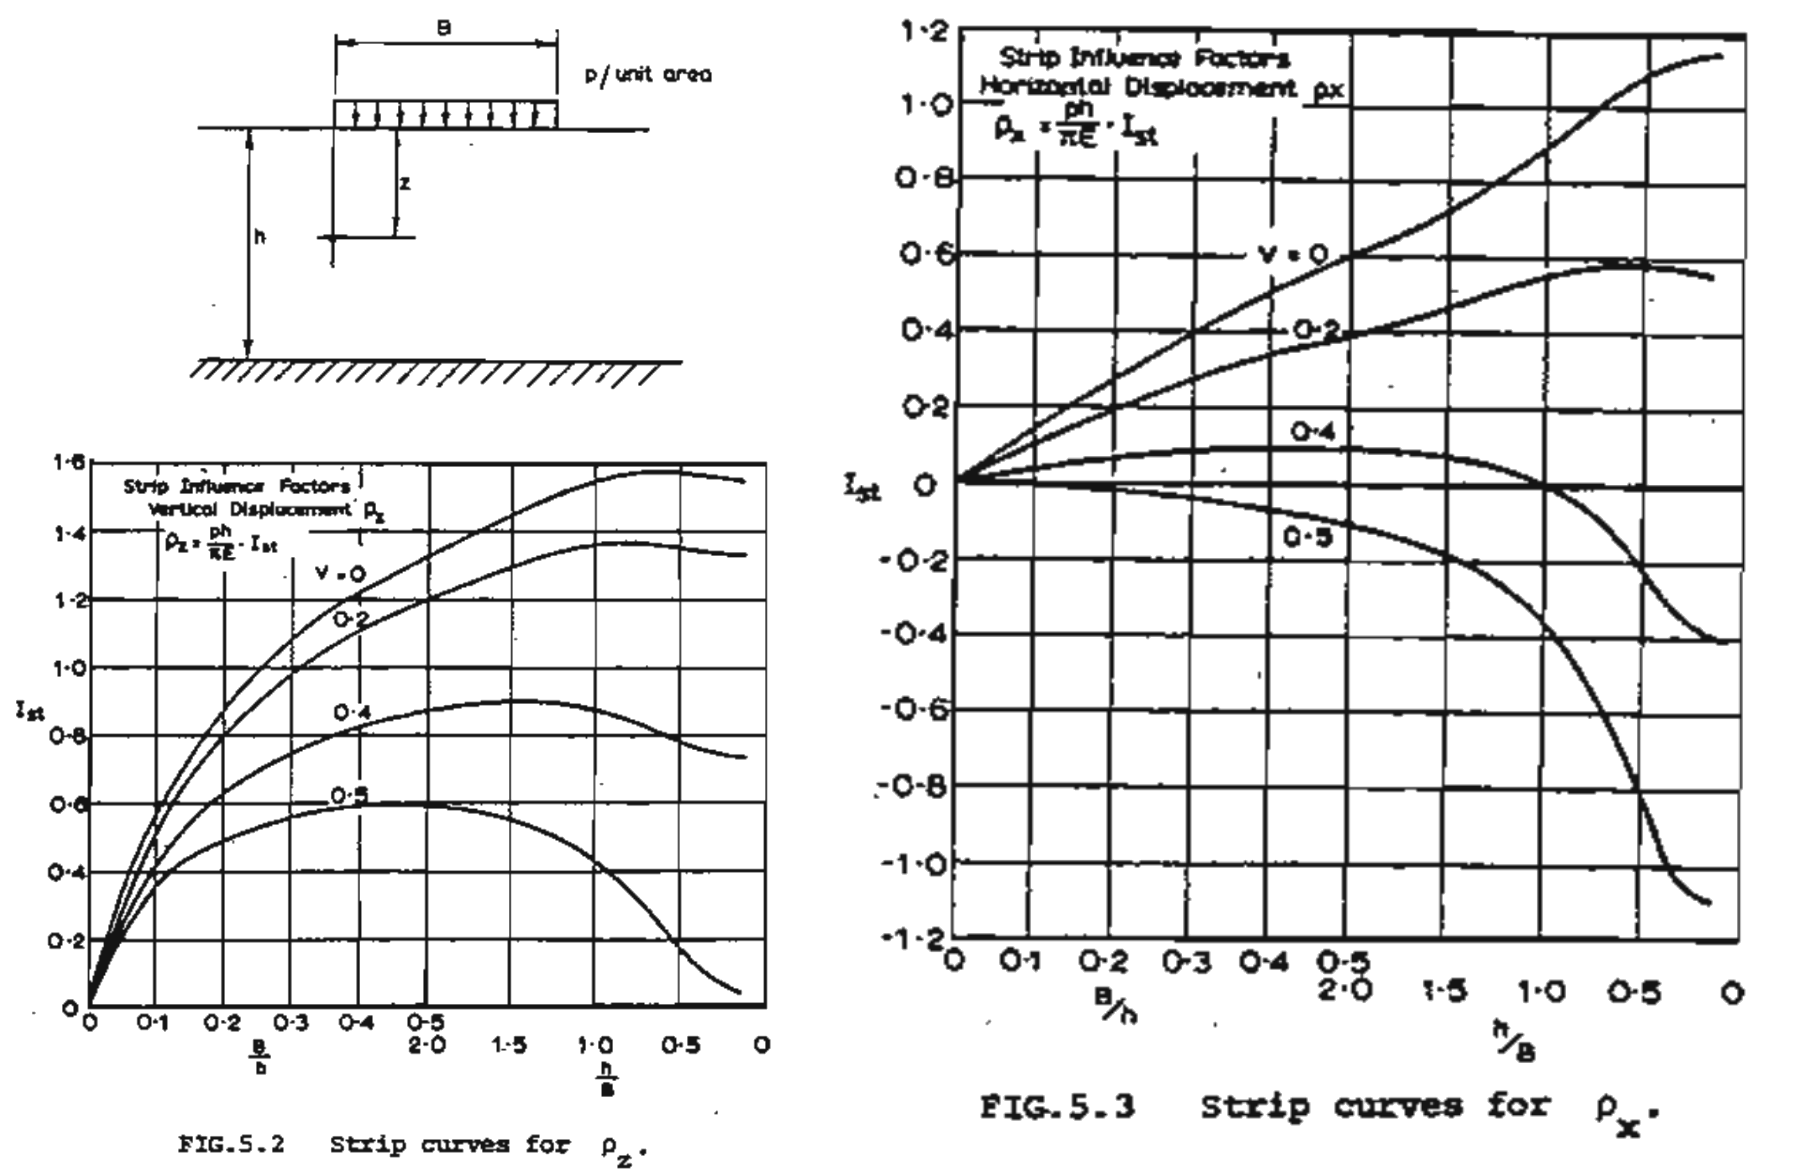
\includegraphics[width=\textwidth]{figs/elasticity-foundation.png}
	\end{figure}
\end{frame}

%----------------------------------------------------------------------------------------
\begin{frame}
\frametitle{Elastic solutions}
	\begin{enumerate}
		\item \textit{Ease of use} Only two parameters, choose equivalent values representative of stran/stress levels.
		\item \textit{Disadvantage}: No failure criteria.
		\item Validate code with chart solutions (``\textit{Exact solutions}")., e.g., Poulos and Davis (1974).
		\item Useful to get feeling of problem (low stress levels) not wide distribution of plastic zones.
	\end{enumerate}
\end{frame}


\section{Soil engineering properties}
%----------------------------------------------------------------------------------------
\begin{frame}
	\frametitle{Stiffness: small to large strains}
	\begin{figure}
		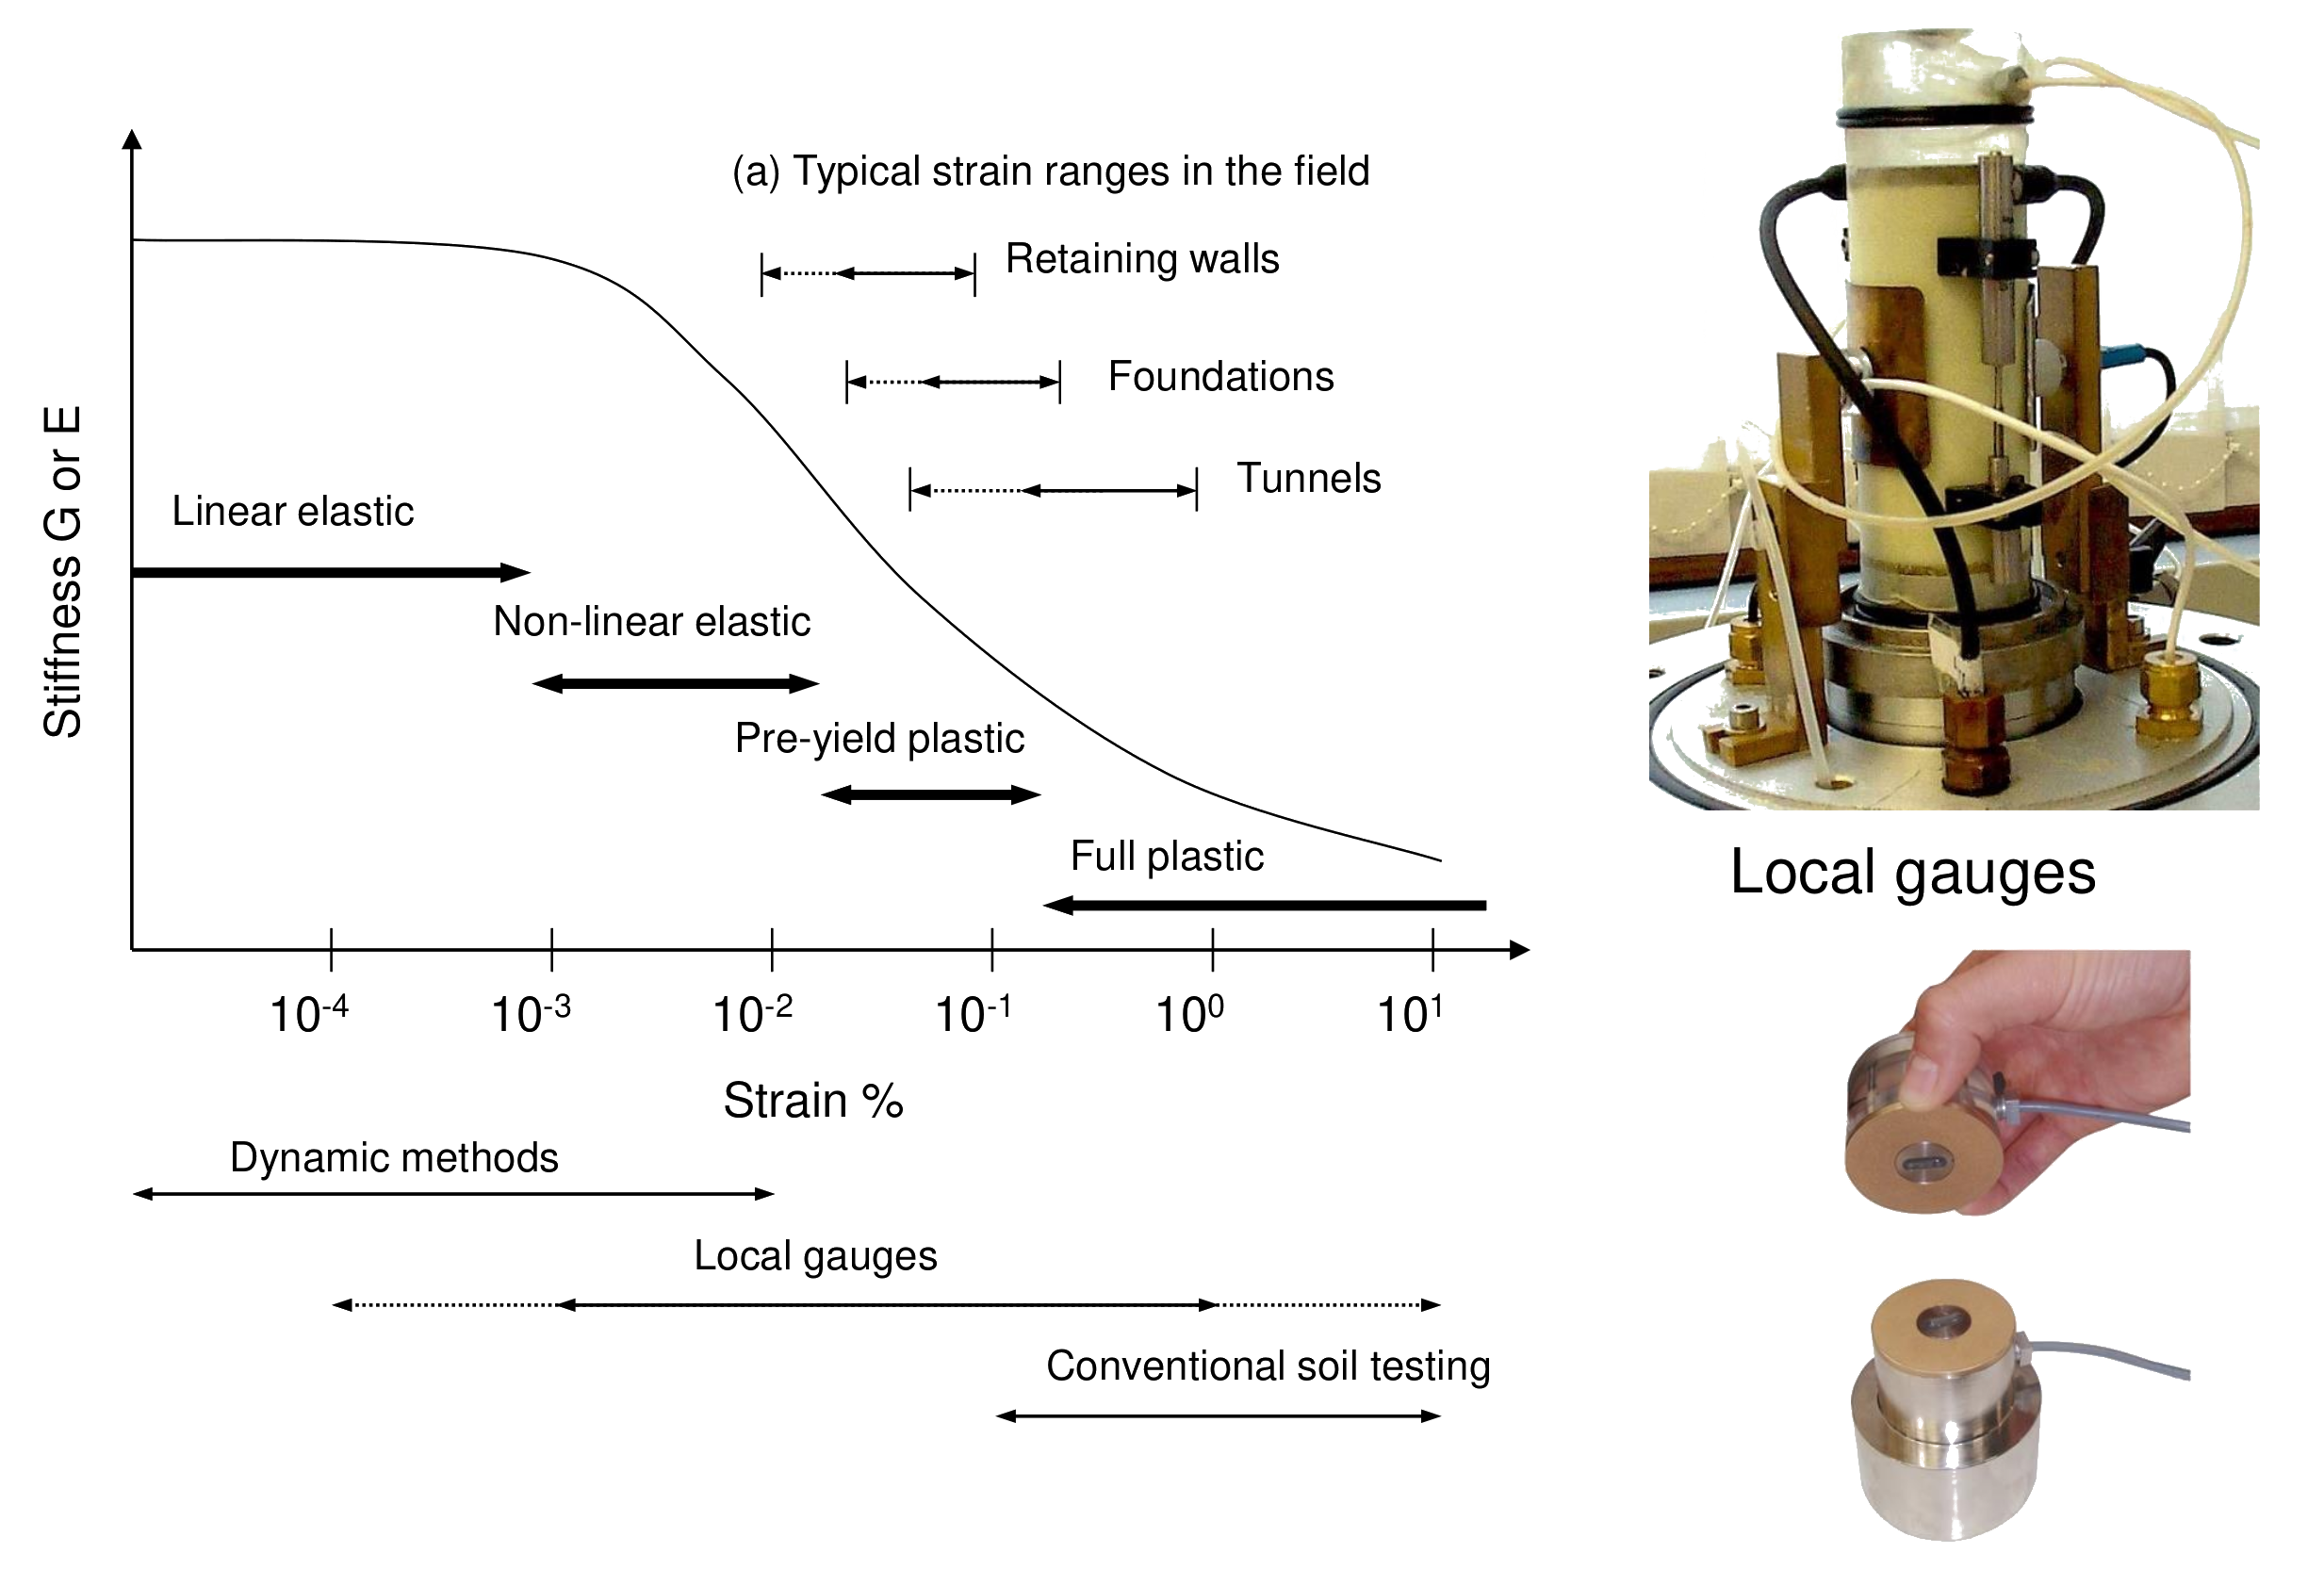
\includegraphics[width=0.9\textwidth]{figs/stiffness-strains.png}
		\caption*{Bender element (GDS)}
	\end{figure}
\end{frame}

%----------------------------------------------------------------------------------------
\begin{frame}
	\frametitle{Stiffness: small to large strains}
	\begin{figure}
		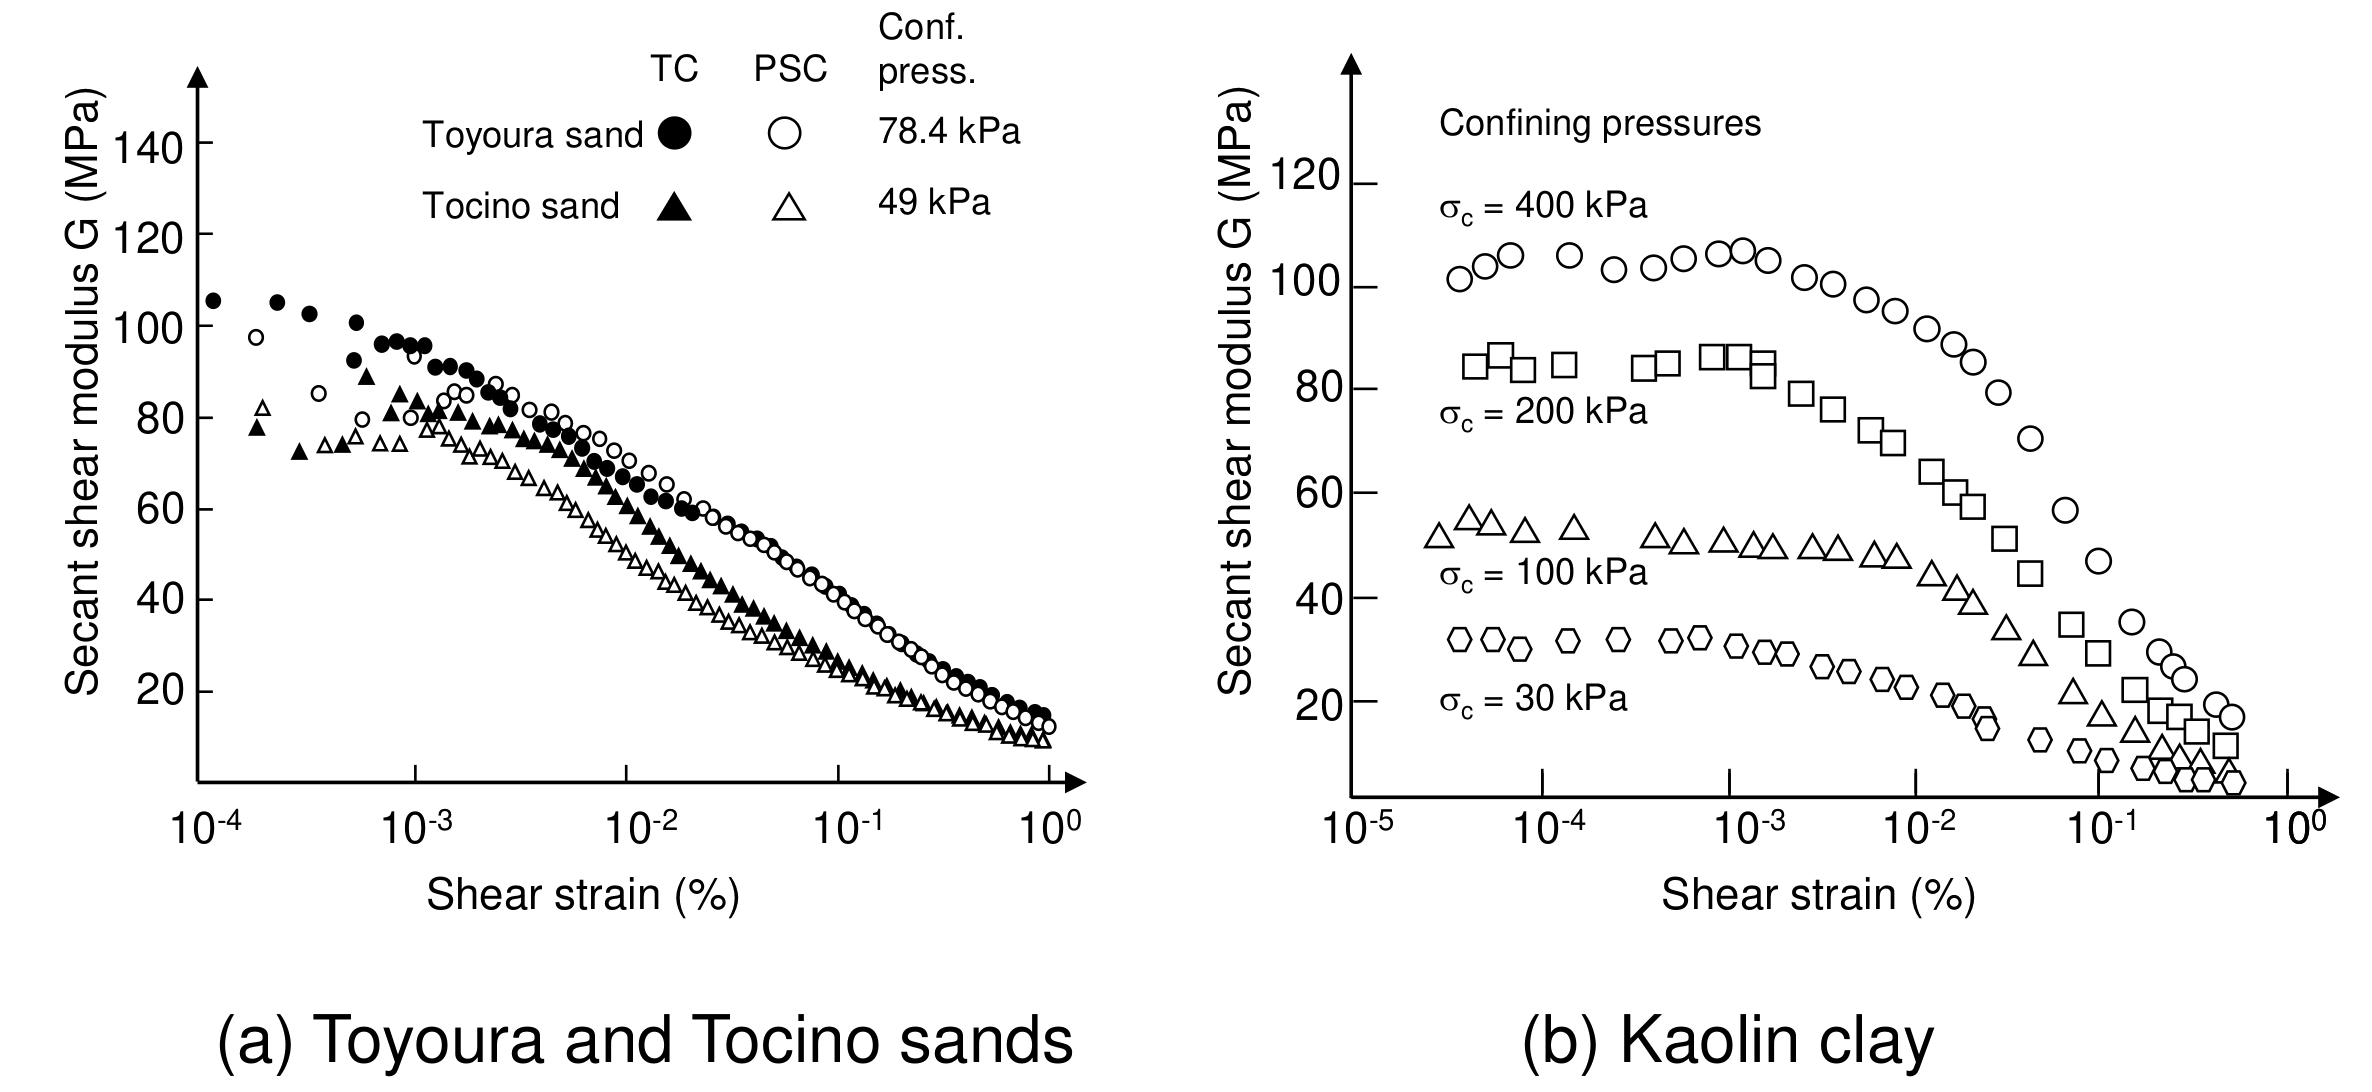
\includegraphics[width=\textwidth]{figs/shear-modulus.png}
	\end{figure}
	\mode<beamer>{
		$E$ or $G$ is a function of:
		\begin{enumerate}
			\item confining stress and void ratio (relative density)
			\item strain level
		\end{enumerate}
	}
	\mode<handout>{
		\vspace{2cm}
	}
\end{frame}


%----------------------------------------------------------------------------------------
\begin{frame}
	\frametitle{Stiffness at intermediate strains}
	\begin{figure}
		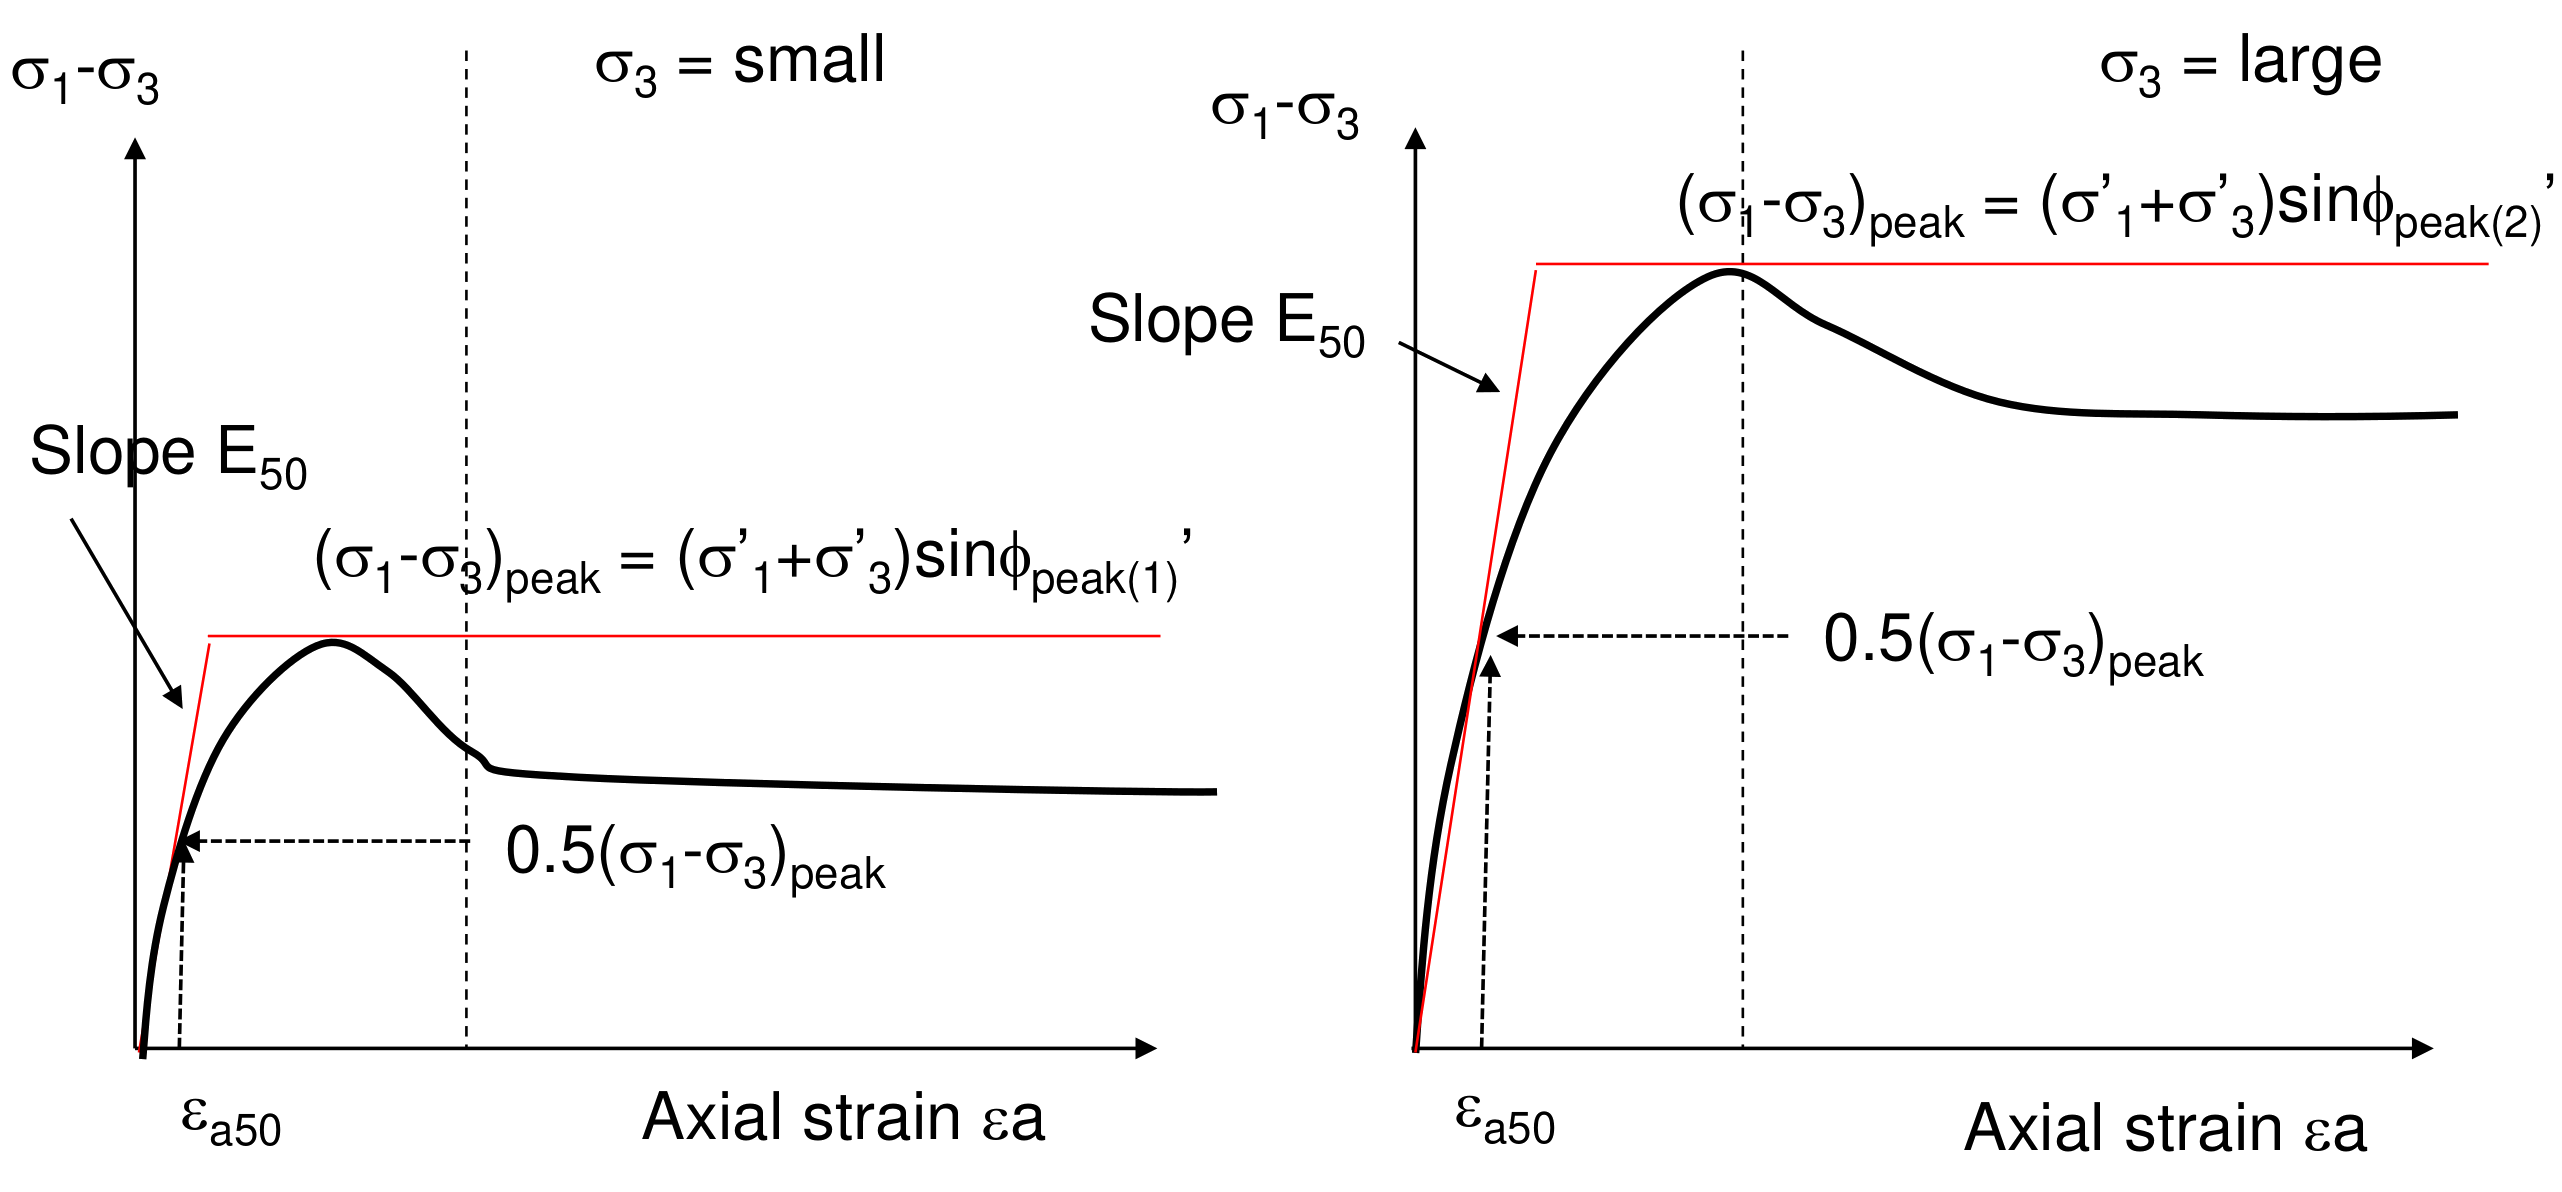
\includegraphics[width=\textwidth]{figs/stiffnes-intermediate-strain.png}
	\end{figure}
	\mode<beamer>{
		$E_{50} = E $ at 50\% of $(\sigma_1 - \sigma_3)_{peak}$
		Note: $\phi_{peak 1}^\prime < \phi_{peak 2}^\prime$
		$E_{50ref} = (0.70 \pm 0.10)E_{oedref}$
	}
	\mode<handout>{
		\vspace{2cm}
	}
\end{frame}

%----------------------------------------------------------------------------------------
\begin{frame}
	\frametitle{Undrained strength}
	\begin{figure}
		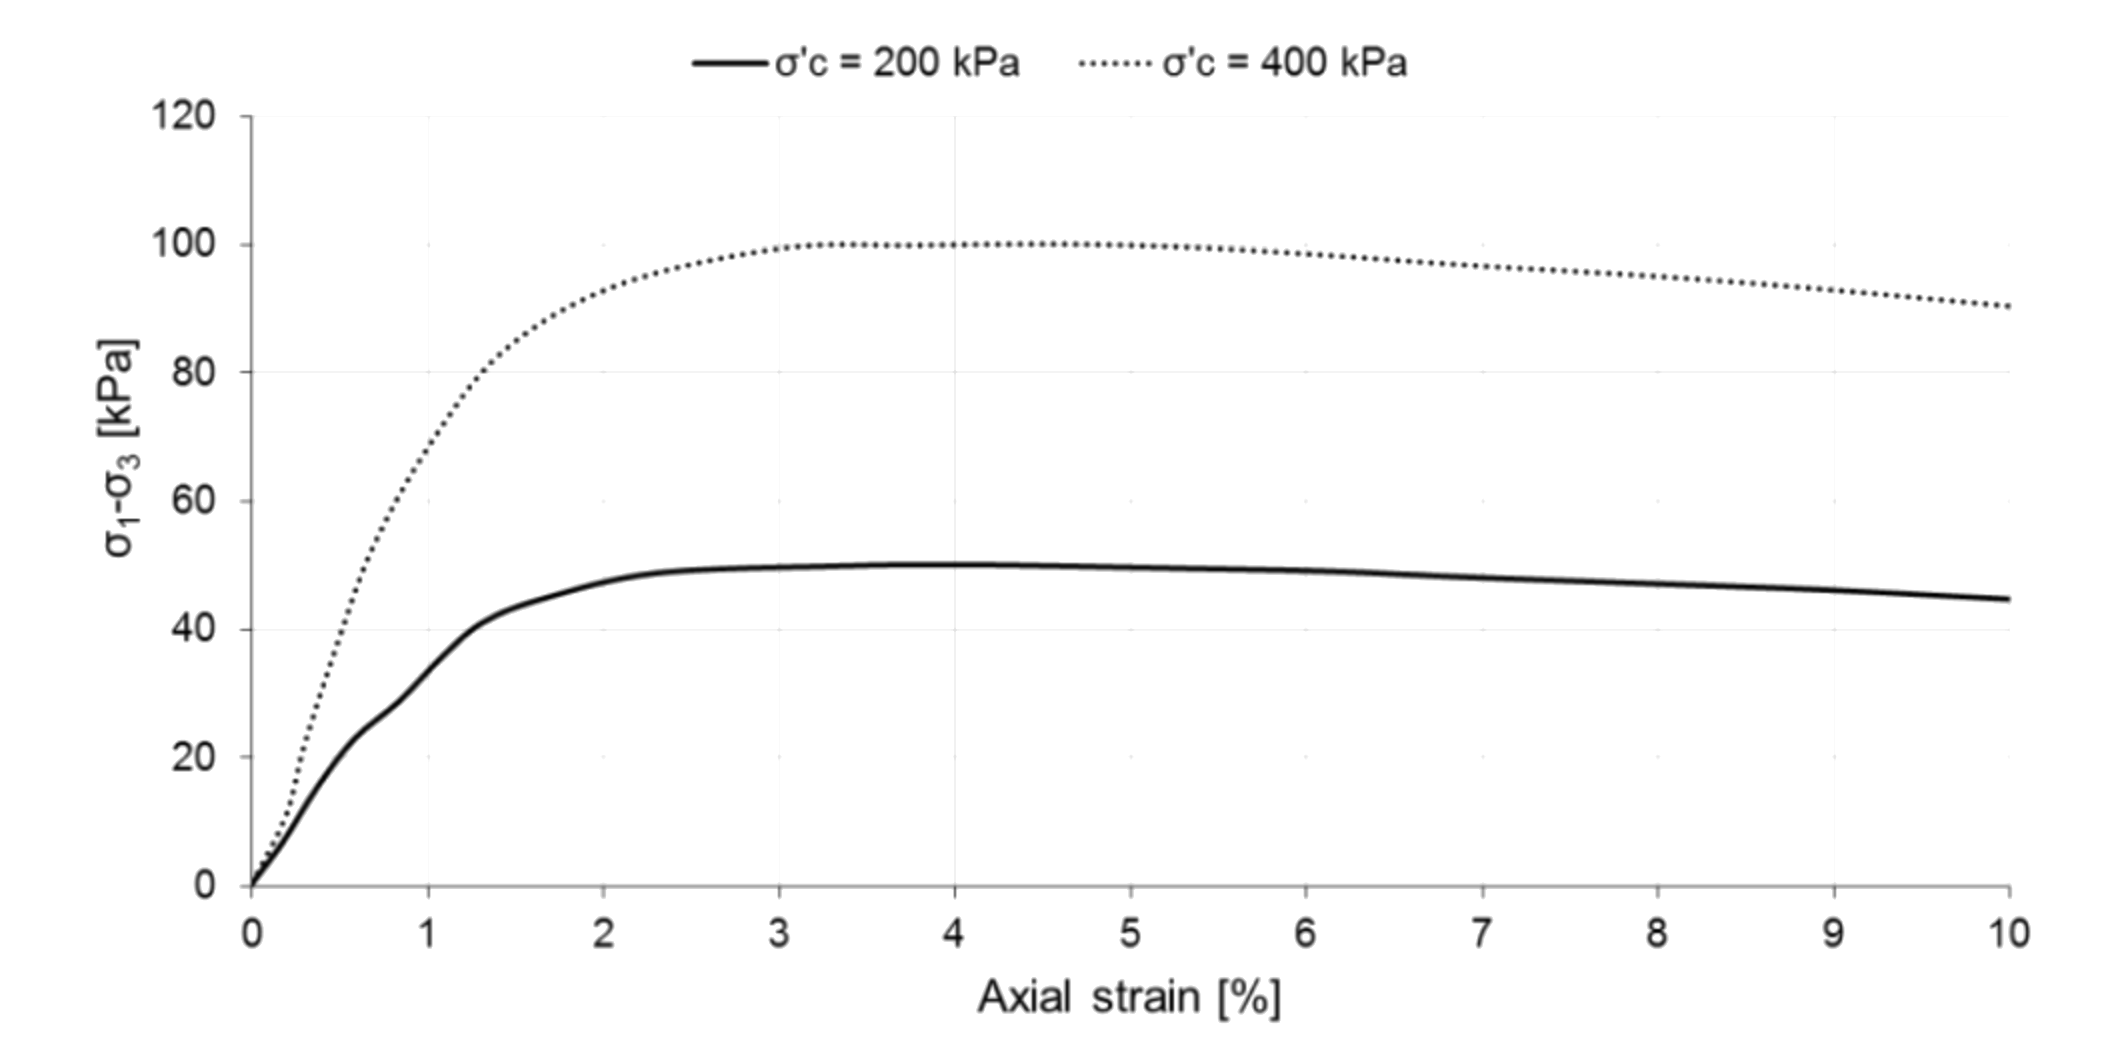
\includegraphics[width=\textwidth]{figs/effect-sigma_c.png}
		\caption*{Triaxial compression test data of homogeneous clay (Ladd \& Foott, 1974)}
	\end{figure}
\end{frame}


%----------------------------------------------------------------------------------------
\begin{frame}
	\frametitle{Normalized undrained strength}
	\begin{figure}
		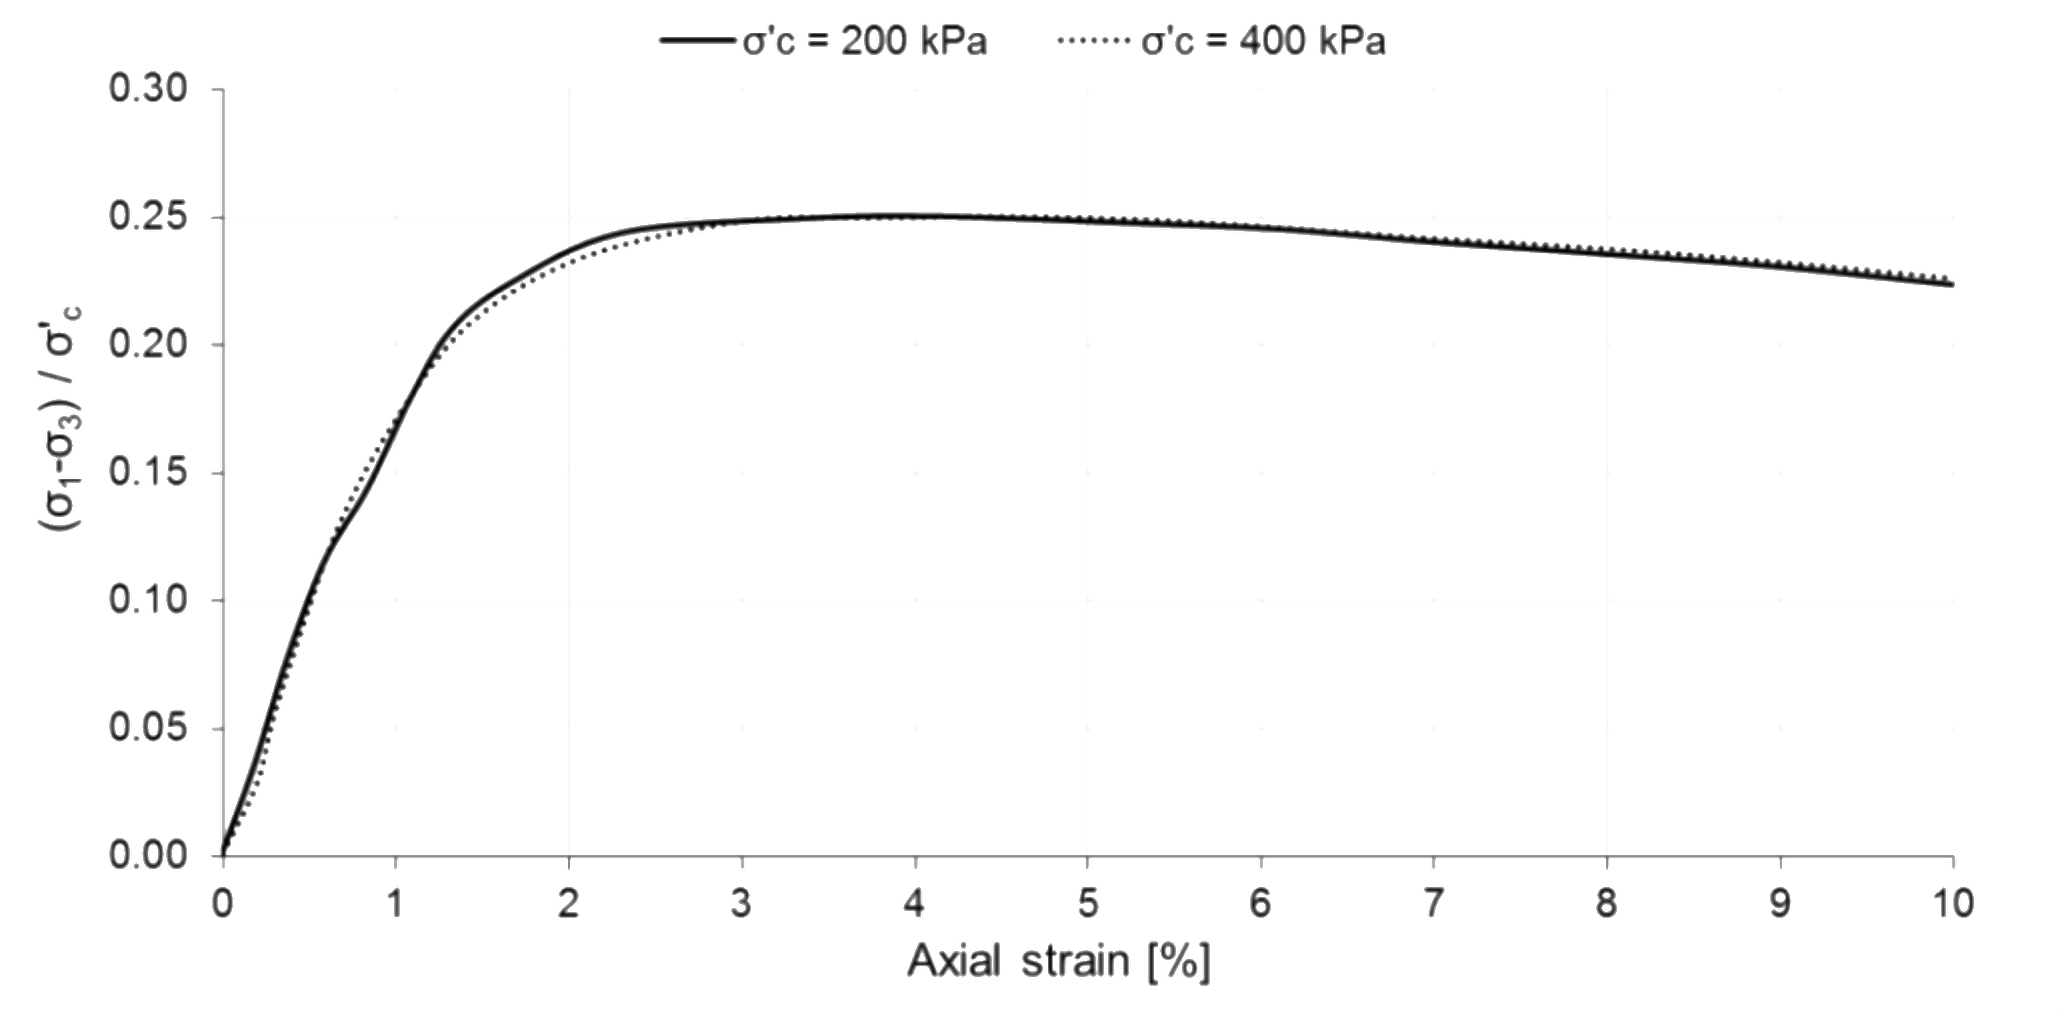
\includegraphics[width=\textwidth]{figs/su_normalised.png}
		\caption*{Normalised triaxial compression test data of homogeneous clay (Ladd \& Foott, 1974)}
	\end{figure}
\end{frame}


%----------------------------------------------------------------------------------------
\begin{frame}
	\frametitle{Stress History and Normalized Soil Engineering Properties (SHANSEP) (Ladd and Foote, 1974)}
	\mode<beamer>{
		\begin{align*}
		(s_u/\sigma_v^\prime) = (s_u/\sigma_v^\prime)_{nc} \times OCR^m \\
		m = 0.8 (0.65 - 0.9)
		\end{align*}
	}
	\mode<handout>{
		\vspace{2cm}
	}
	\begin{figure}
		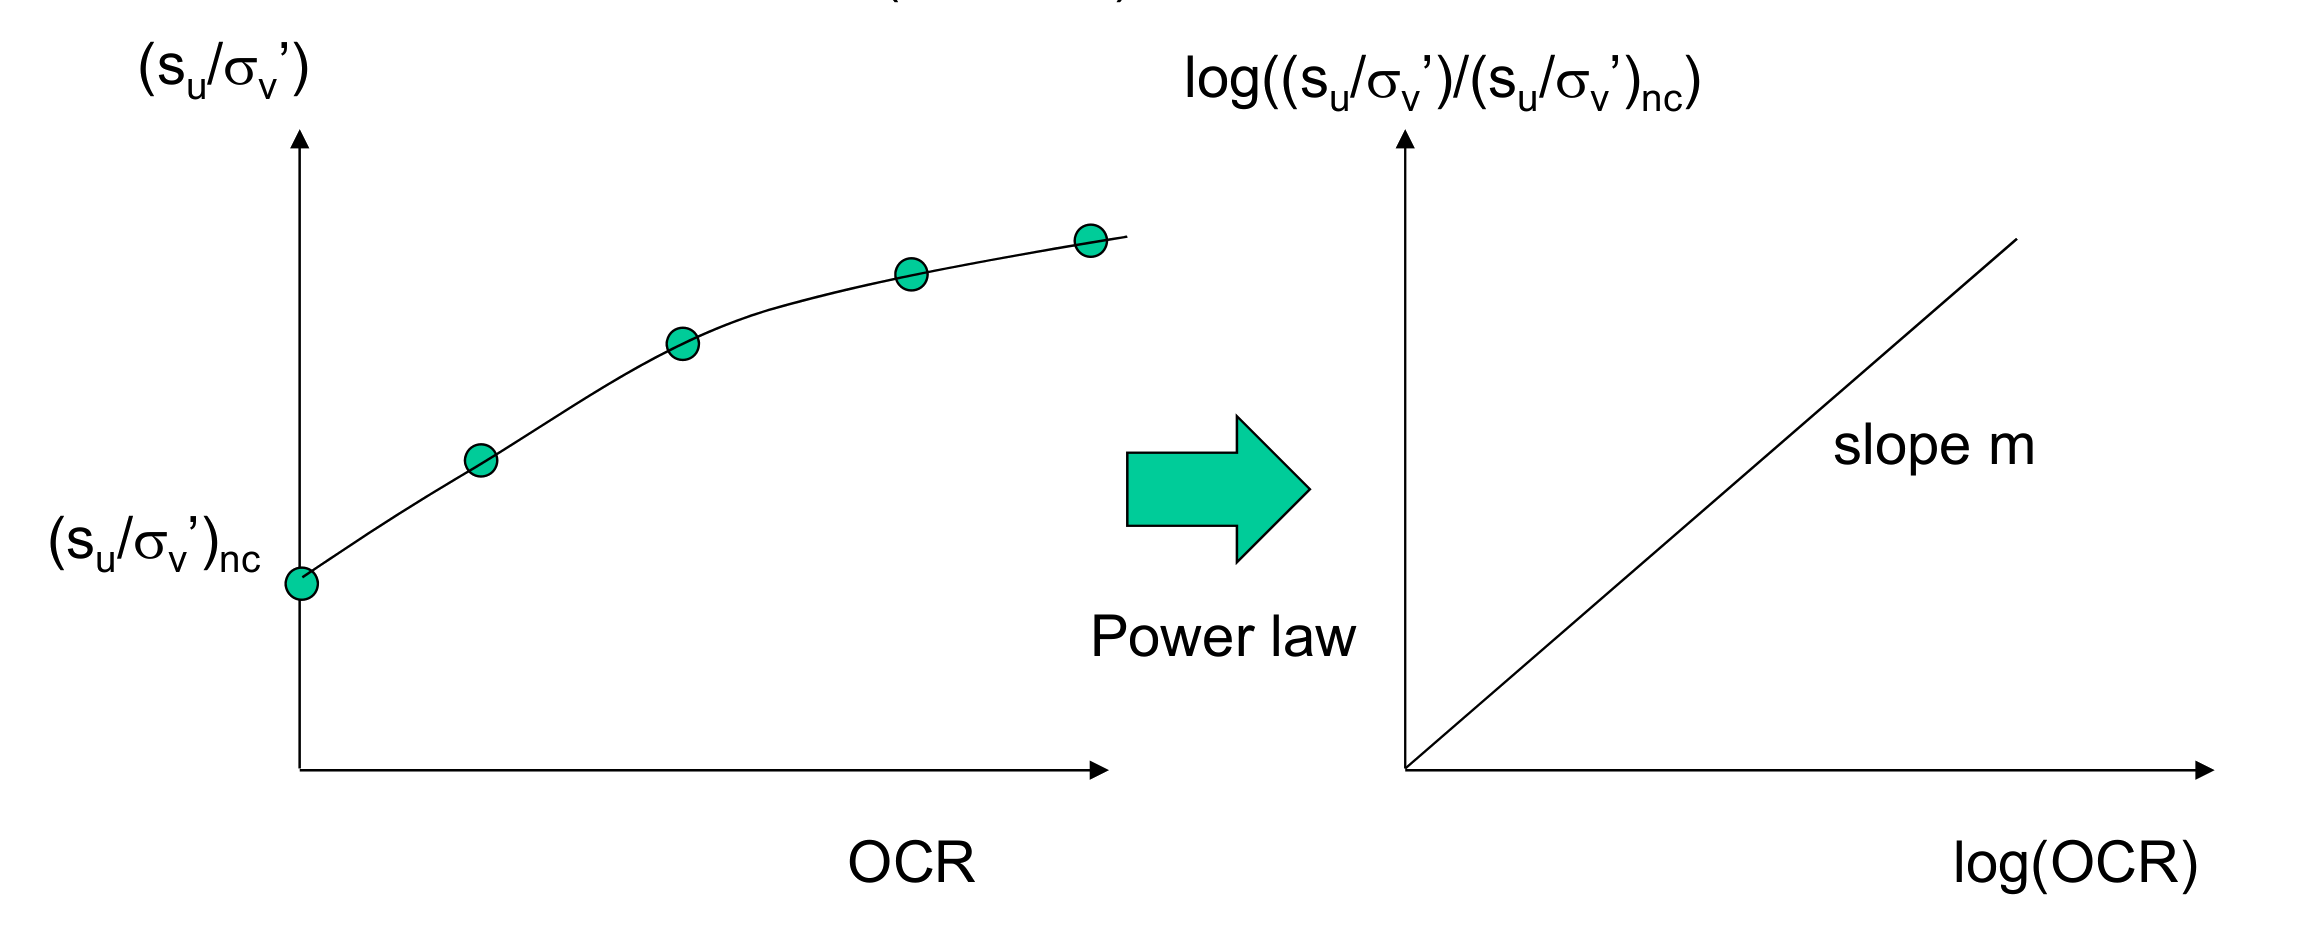
\includegraphics[width=\textwidth]{figs/shansep.png}
	\end{figure}
\end{frame}

\note{
	Laboratory tests conducted at the Imperial College using remolded clays (Henkel (1960)
	and Parry (1960)) and at the Massachusetts Institute of Technology on a wide range of
	clays, give evidence that clay samples with the same over-consolidation ratio (OCR), but
	different consolidation stress $\sigma_c^\prime$ and therefore different pre-consolidation stress $\sigma_{p}^\prime$, exhibit very similar strength and stress-strain characteristics when the results are
	normalized over the consolidation stress $\sigma_c^\prime$.
	
	In practice, normalized behaviour is not as perfect as shown, there is discrepancy in the normalized plots caused by different consolidation stresses, soil deposit heterogeneity or even the fact that the conditions from one soil test to another are not identical. However, this discrepancy is reported to be quite small.
}

%------------------------------------------------
\section{References}
%------------------------------------------------

%----------------------------------------------------------------------------------------
\begin{frame}{Isotropic Linear Elastic Stress-strain relationship}
	The \textit{isotropic tensor} $D_{ijkl}$:
	\begin{equation*}
	D_{ijkl} = \lambda \delta_{ij}\delta_{kl} + \mu (\delta_{ik}\delta_{jl} + \delta_{il}\delta_{jk}) + \alpha (\delta_{ik}\delta_{jl} - \delta_{il}\delta_{jk})
	\end{equation*}
	Where $\lambda, \mu, \text{ and }, \alpha$ are scalar constants. Since $D_{ijkl}$ must satisfy symmetry, $\alpha = 0$.
	\mode<beamer>{
		\begin{equation*}
		D_{ijkl} = \lambda \delta_{ij}\delta_{kl} + \mu (\delta_{ik}\delta_{jl} + \delta_{il}\delta_{jk})
		\end{equation*}
	}
	\mode<handout>{
		\vspace{1cm}
	}
	So the stress:
	\mode<beamer>{
		\begin{align*}
		\sigma_{ij} & = \lambda \delta_{ij}\delta_{kl}\varepsilon_{kl} + \mu (\delta_{ik}\delta_{jl} + \delta_{il}\delta_{jk})\varepsilon_{kl}\\
		\sigma_{ij} & = \lambda \varepsilon_{kk} \delta_{ij} + 2\mu \varepsilon_{ij}
		\end{align*}
	}
	\mode<handout>{
		\vspace{2.5cm}
	}
	Hence for an isotropic linear elastic material, there are only two independent material constants, $\lambda$ and $\mu$, which are called \textit{Lame's constants}.
\end{frame}

%----------------------------------------------------------------------------------------
\begin{frame}{SHANSEP procedure}
	\mode<beamer>{
		\begin{figure}
			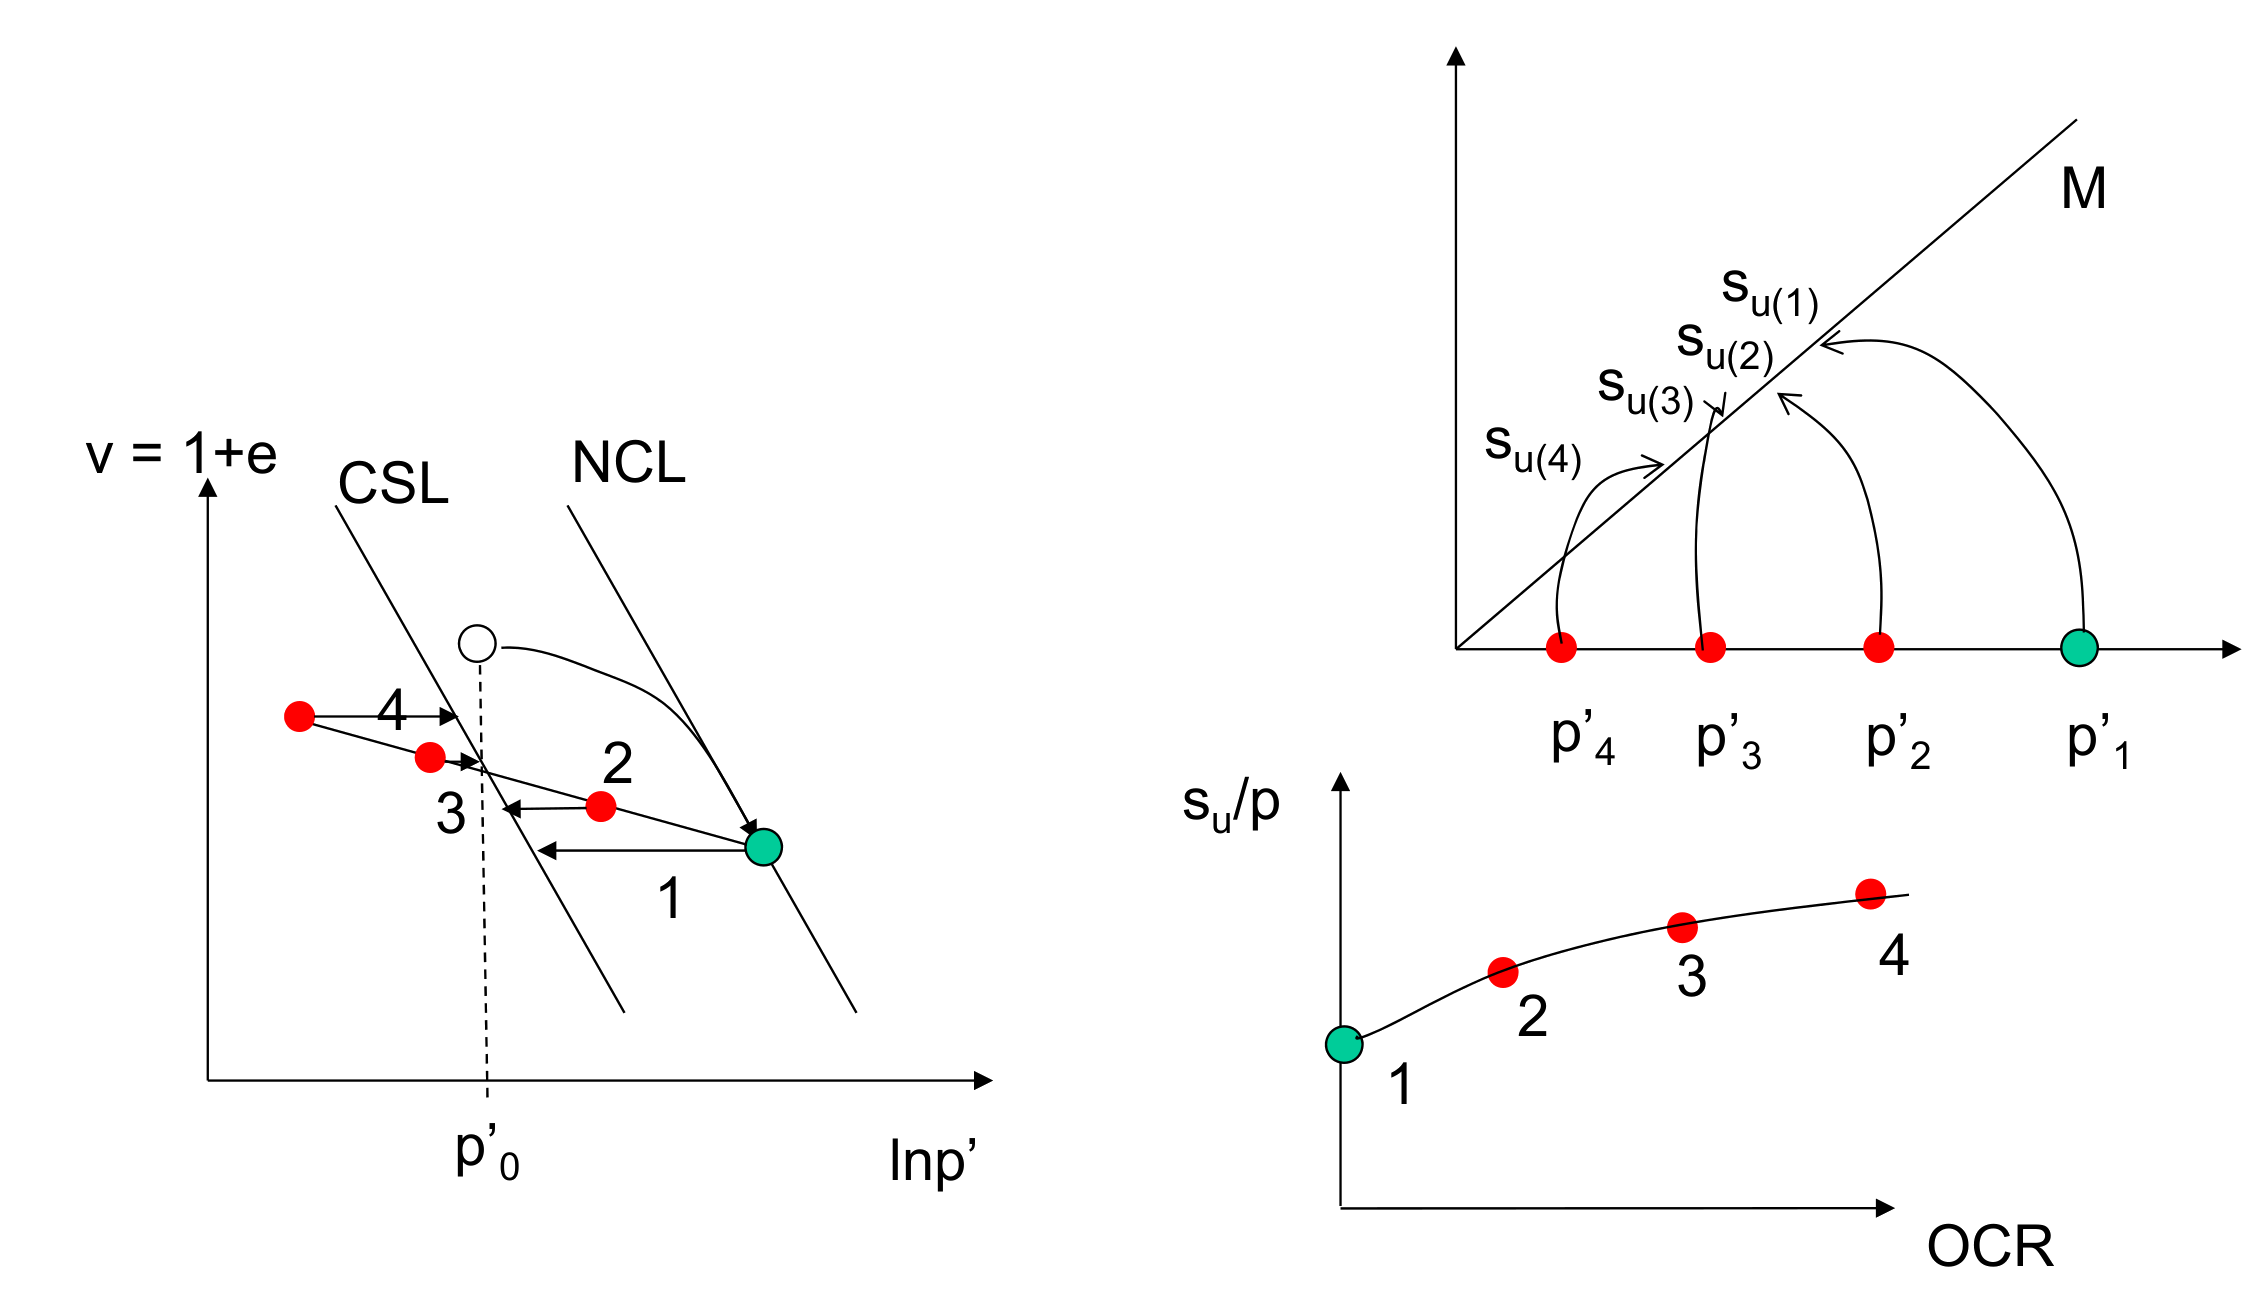
\includegraphics[width=\textwidth]{figs/shansep-procedure.png}
		\end{figure}
	}
	\mode<handout>{
		\vspace{6cm}
	}
\end{frame}
\note{
	\begin{enumerate}
		\item obtain a sample of “clayey” soil
		\item Reconsolidate to 1.5 to 2.0 of insitu effective mean pressure $p^\prime_0$ , or
		reconsolidate back to the virgin normal compression line
		\item Rebound to desired OCR
		\item Perform undrained shearing and find $s_u$ .
		\item Perform multiple tests at different OCRs.
		\item Evaluate 	$(s_u/\sigma_v^\prime) = (s_u/\sigma_v^\prime)_{nc} \times OCR^m$
	\end{enumerate}
}

\end{document}
